\documentclass{article}
\usepackage[a4paper]{geometry}
\usepackage[utf8]{inputenc}
\usepackage[french]{babel}

\usepackage{graphicx}
\usepackage{courier}
\usepackage{listings}

\usepackage[svgnames]{xcolor}
\xdefinecolor{darkgreen}{named}{DarkGreen}

\lstdefinelanguage{lustre}{%
   columns=fullflexible,%
   basicstyle=\tt\footnotesize,
   % keywordstyle=\bfseries,
   commentstyle=\slshape,%
   keywords={%
     node,var,let,tel,returns,
     when,merge
   },%
   keywordstyle={\color{darkgreen}\sffamily},%
   morekeywords=[2]{%
     int, real, bool,
   },%
   keywordstyle=[2]{\color{blue}\ttfamily},%
   classoffset=2,%
   morekeywords=[3]{%
     storage, parameter, code %
   },%
   morekeywords=[3]{
     True,False
   },
   keywordstyle=[3]{\color{purple}},%
   sensitive,%
   morestring=[d]",%"
}[keywords,comments,strings]%

\lstMakeShortInline[language=albert]?

\lstset{language=lustre}

\title{Parallélisme Synchrone\\ Réalisation d'un compilateur pour Minilucy}
\author{Basile Pesin}
\date{\today}

\begin{document}

\maketitle

\section{Choix techniques}

\subsection{Choix de langage}

Pour des raisons de simplicité (et de familiarité), on a décidé d'implémenter le compilateur pour MiniLucy dans le langage OCaml. Ce langage fonctionnel est parfaitement adapté à la manipulation d'arbres de syntaxes abstraits. On l'a préféré au langage pur Haskell pour ce projet, afin de simplifier la gestion des exceptions (qui peuvent être gérées entièrement dynamiquement en OCaml). En dehors des exceptions, on a en revanche essayé d'écrire le compilateur dans le style le plus ``pur'' possible, en particulier en évitant les entrées-sorties, et autres effets de bord dans les fonctions internes, pour plutôt les réaliser dans la fonction ``main'' du compilateur.

\subsection{Manuel d'utilisation}

Le compilateur peut être facilement compilé grâce à la commande \textit{make}. Le fichier exécutable \texttt{minilucy.byte} est alors généré. Le logiciel ne présente pas de dépendance particulière, en dehors du compilateur \texttt{ocaml}, de \texttt{menhir} et d'\texttt{ocamllex}. Compiler le compilateur déclenche aussi la compilation des exemples (qui peut être déclenchée séparément avec \textit{make samples}), en mode ``assert'' du compilateur Minilucy (décrit plus bas).

\paragraph{Options du compilateur}

Les options suivantes peuvent être passées au compilateur \texttt{minilucy}:

\begin{itemize}
  \item \textit{-parse}, \textit{-desugar}, \textit{-check}, \textit{-norm}, \textit{-translate}, \textit{-generate} permettent respectivement d'arrêter la compilation après le parsing, l'élimination du sucre syntaxique, la vérification statique, la normalisation (et ordonnancement), la traduction vers \texttt{Obc}, et la génération de code \texttt{C}. Dans tous les cas, le compilateur affichera alors le programme compilé à cette étape.
  \item \textit{-asserts} permet d'activer les vérifications de correctitude du compilateur. Celles-ci sont décrites plus en détail dans la section \ref{compilVerif}.
  \item \textit{-interpet k node} permet d'utiliser l'interpréteur (voir \ref{interpreter}) pour exécuter \textit{k} itérations d'une \textit{node} spécifiée. Le programme affiche alors les flots de sorties de la \textit{node} après les \textit{k} itérations.
\end{itemize}

\subsection{Architecture du compilateur}

Pour structurer les différentes passes du compilateur, on a suivi de manière assez proche l'article \cite{Biernacki08}. La figure \ref{fig:passesCompil} récapitule les langages intermédiaires utilisés, ainsi que les passes de compilations permettant de passer de l'une à l'autre.

\begin{figure}[!ht]
  \centering
  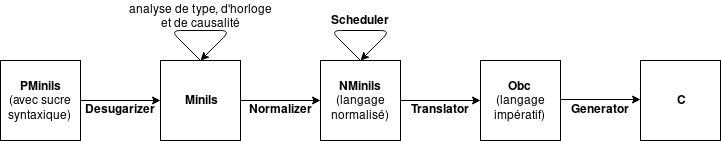
\includegraphics[width=.7\paperwidth]{assets/chain.png}
  \caption{Passes de compilation}
  \label{fig:passesCompil}
\end{figure}

\section{Extensions}

\subsection{Polymorphisme d'horloge}

La première (légère) extension réalisée est un ajout par rapport aux règles de typages données dans~\cite{Biernacki08}. En effet, les règles de typages d'horloge données par l'article exigent que toutes les flux d'entrées (et de sortie) d'une application soient sur la même horloge. On décide dans cette extension de relaxer cette contrainte, en introduisant une notion de ``polymorphisme'' d'horloge lors de l'appel à une node.

On va pour cela profiter de la syntaxe de l'appel de fonction dans notre langage, qui permet de préciser une expression de \texttt{every} pour tout appel de node. On infère l'horloge qui sera l'horloge de base de la node interne (celle sur laquelle celle-ci sera exécutée) en unifiant les horloges de retour attendues, avec les horloges de retour déclarées pour la node. On compose ensuite cette horloge de base avec les horloge des paramètres formels de la node, pour obtenir les horloges des paramètres passés, qu'on doit alors vérifier. Par exemple, le typage d'horloge des nodes suivantes est accepté.

\begin{lstlisting}
node test_op(b : bool) returns (z : int when True(b));
let
  z = 3 when True(b);
tel;

node test_app(b1 : bool; c1 : bool) returns (z : int when True(c1) when True(b1));
let
  z = test_op(b1 when True(c1));
tel;
\end{lstlisting}

\subsection{Automates}

Dans une extension plus importante, on ajoute les automates à état au langage, en s'inspirant de~\cite{Colaco05}. On donne ci-dessous un exemple d'automate.

\begin{lstlisting}
node auto_simpl() returns (x : int);
let
  automaton
  | INC ->
    let u : int = (1 + pre u) in
    x = 0 fby x + u;
    until x > 5 then DEC;
  | DEC ->
    let u : int = 2 in
    x = 0 fby x - u;
    until x < -10 then INC;
  end;
tel;
\end{lstlisting}

Toute équation doit être définie dans tous les états de l'automate. En revanche, on donne aussi au programmeur la possibilité de définir des variables locales à l'un des état (via le \lstinline[mathescape]{let $\ldots$ in}). Il est également possible de définir des automates imbriqués (plus d'exemples sont disponibles dans le fichier \texttt{samples/automatatest.lus}).

Les automates sont compilés depuis le langage parsé vers le langage noyau (ils ne perturbent donc pas les étapes suivantes de compilation). La compilation des automates utilise très fortement le système d'horloge n-aire du langage : typiquement, une horloge est introduite par automate, avec un constructeur pour chacun de ses états. Les instructions \lstinline{until} permettent de faire varier la valeur de cette horloge (et donc opèrent les transitions de l'automate).

Une autre caractéristique importante des automates est le \lstinline{reset} : lors du changement d'état d'un automate, toutes les équations déclarées par cet état sont réinitialisées, c'est à dire que dans le cas d'un \lstinline{fby}, on reprends à la valeur initiale (les nodes appelées en interne sont également réinitialisées). Ce trait est également implémenté comme dans l'article~\cite{Colaco05}, mais sans construction \lstinline{reset} explicite.

\subsection{Interpréteur}
\label{interpreter}

Afin de pouvoir tester les nodes écrites sans avoir à compiler l'entièreté du programme, on a développé un interpréteur pour les programmes du langage noyau. Celui ci travaille sur des flots non-bornés (l'interpréteur garde en mémoire l'historique entier de chaque flot, ce qui n'est pas si grave puisqu'il est destiné à être en pratique utilisé pour tester un noeud sur un petit nombre d'itérations). L'interpréteur peut alors implémenter une sémantique relativement simple. Par ailleurs, l'interpréteur étant exécuté avant les phases de vérifications statiques (de type, d'horloge et de causalité), il permet éventuellement d'évaluer des programmes faux (mais peut aussi échouer sur de tels programmes). 

On a également défini un interprète étendu, qui s'exécute sur le langage enrichi d'automates (et de quelques autres éléments de sucre syntaxique). Cet interpréteur implémente donc une sémantique d'automate (encore une fois, avec des flots non-bornés). On utilisera ce deuxième interpréteur dans la section \ref{compilVerif}.

\subsection{Vérification des phases de compilation}
\label{compilVerif}

Afin de se donner une meilleure confiance dans le compilateur, on a développé plusieurs phases de vérifications, qui permettent de s'assurer (de manière dynamique) que les transformations réalisées sur un programme sont correctes. Ces vérifications peuvent être activées avec l'option \texttt{-asserts} du compilateur.

\paragraph{Traduction des automates}
Cette première vérification était la plus complexe à mettre en place. C'est en effet pour pouvoir l'effectuer qu'on a développé les interpréteur décrits dans la section \ref{interpreter}. Une fois ces deux interpréteurs développés (un pour le langage noyau, un pour le langage étendu), il suffit cela dit de les exécuter sur les programmes avant et après élimination du sucre syntaxique, et de comparer les résultats. On effectue pour le moment ces tests avec des entrées aléatoires choisies uniformément, mais développer une génération plus ``utile'' de ces entrées serait un problème intéressant.

\paragraph{Normalisation}
Etant donné que la normalisation consiste principalement en la séparation des équations utilisant des états en plusieurs équations, la vérification de l'équivalence des deux programmes peut se faire simplement en ré-inlinant les équations séparées, et en vérifiant que les ensembles d'équations obtenues sont équivalents.

\paragraph{Ordonnancement}
La vérification de la phase d'ordonnancement est la plus simple de toutes, puisqu'il suffit de vérifier que les équations sont bien ordonnancées, c'est à dire que tout flot utilisé par une équation est déclaré par l'une des équations précédentes.

\paragraph{Traduction} Etant donné que la phase de traduction transforme le programme Lustre normalisé en un tout nouveau langage (Obc), il est difficile de réaliser une vérification qui soit significativement plus simple que la transformation elle-même. On se contente donc pour cette phase de vérifier que toutes les entrées et sorties sont bien similaires à celles du programme non-traduit, et que les sorties et variables locales sont bien toutes déclarées par les instructions de la machine. Cette vérification pourrait éventuellement être renforcée par un nouvel interpréteur, mais on n'a pas pu en réaliser un pour des raisons de temps.

\subsection{AVR-Lustre}

Comme le compilateur réalisé génère du code C, pourquoi ne pas en profiter pour cibler des microcontrôleurs pouvant être programmés en C ? En effet, les microcontrôleurs étant au coeur des systèmes embarqués pour lesquelles la programmation synchrone est souvent utilisée, ce portage semble particulièrement adapté.

On a choisi pour ce Proof of Concept de cibler l'architecture AVR, en particulier utilisée sur les microcontrôleurs de la gamme Arduino. On a spécifiquement paramétré une petite bibliothèque d'exécution (tirée de celle de la machine virtuelle OMicroB~\cite{VVC18}) pour utiliser les ports de la carte Arduino Uno (la plus commune de la gamme Arduino). De plus, on a écrit une petite bibliothèque supplémentaire, inspirée de celle fournit par Arduino, pour pouvoir piloter un écran LCD externe.

Grâce à cet ensemble de fonctionnalité, on a pu implémenter l'exemple du chronomètre présenté dans l'article~\cite{Colaco05} en tant que système physique.

\bibliography{biblio}{}
\bibliographystyle{unsrt}

\end{document}
